% Created by tikzDevice version 0.10.1 on 2016-08-26 10:15:03
% !TEX encoding = UTF-8 Unicode
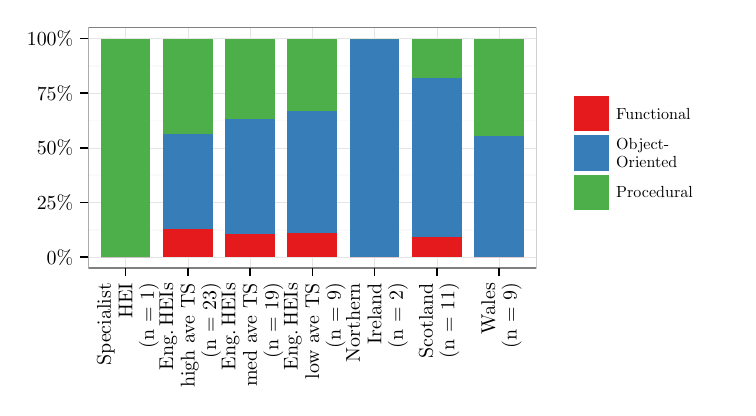
\begin{tikzpicture}[x=1pt,y=1pt]
\definecolor{fillColor}{RGB}{255,255,255}
\path[use as bounding box,fill=fillColor,fill opacity=0.00] (0,0) rectangle (252.94,130.09);
\begin{scope}
\path[clip] (  0.00,  0.00) rectangle (252.94,130.09);
\definecolor{drawColor}{RGB}{255,255,255}
\definecolor{fillColor}{RGB}{255,255,255}

\path[draw=drawColor,line width= 0.6pt,line join=round,line cap=round,fill=fillColor] (  0.00,  0.00) rectangle (252.94,130.09);
\end{scope}
\begin{scope}
\path[clip] ( 21.89, 43.19) rectangle (183.84,130.09);
\definecolor{fillColor}{RGB}{255,255,255}

\path[fill=fillColor] ( 21.89, 43.19) rectangle (183.84,130.09);
\definecolor{drawColor}{gray}{0.98}

\path[draw=drawColor,line width= 0.6pt,line join=round] ( 21.89, 57.02) --
	(183.84, 57.02);

\path[draw=drawColor,line width= 0.6pt,line join=round] ( 21.89, 76.76) --
	(183.84, 76.76);

\path[draw=drawColor,line width= 0.6pt,line join=round] ( 21.89, 96.51) --
	(183.84, 96.51);

\path[draw=drawColor,line width= 0.6pt,line join=round] ( 21.89,116.26) --
	(183.84,116.26);
\definecolor{drawColor}{gray}{0.90}

\path[draw=drawColor,line width= 0.2pt,line join=round] ( 21.89, 47.14) --
	(183.84, 47.14);

\path[draw=drawColor,line width= 0.2pt,line join=round] ( 21.89, 66.89) --
	(183.84, 66.89);

\path[draw=drawColor,line width= 0.2pt,line join=round] ( 21.89, 86.64) --
	(183.84, 86.64);

\path[draw=drawColor,line width= 0.2pt,line join=round] ( 21.89,106.39) --
	(183.84,106.39);

\path[draw=drawColor,line width= 0.2pt,line join=round] ( 21.89,126.14) --
	(183.84,126.14);

\path[draw=drawColor,line width= 0.2pt,line join=round] ( 35.38, 43.19) --
	( 35.38,130.09);

\path[draw=drawColor,line width= 0.2pt,line join=round] ( 57.88, 43.19) --
	( 57.88,130.09);

\path[draw=drawColor,line width= 0.2pt,line join=round] ( 80.37, 43.19) --
	( 80.37,130.09);

\path[draw=drawColor,line width= 0.2pt,line join=round] (102.86, 43.19) --
	(102.86,130.09);

\path[draw=drawColor,line width= 0.2pt,line join=round] (125.36, 43.19) --
	(125.36,130.09);

\path[draw=drawColor,line width= 0.2pt,line join=round] (147.85, 43.19) --
	(147.85,130.09);

\path[draw=drawColor,line width= 0.2pt,line join=round] (170.34, 43.19) --
	(170.34,130.09);
\definecolor{fillColor}{RGB}{228,26,28}

\path[fill=fillColor] ( 26.39, 47.14) rectangle ( 44.38, 47.14);
\definecolor{fillColor}{RGB}{55,126,184}

\path[fill=fillColor] ( 26.39, 47.14) rectangle ( 44.38, 47.14);
\definecolor{fillColor}{RGB}{77,175,74}

\path[fill=fillColor] ( 26.39, 47.14) rectangle ( 44.38,126.14);
\definecolor{fillColor}{RGB}{228,26,28}

\path[fill=fillColor] ( 48.88, 47.14) rectangle ( 66.87, 57.44);
\definecolor{fillColor}{RGB}{55,126,184}

\path[fill=fillColor] ( 48.88, 57.44) rectangle ( 66.87, 91.79);
\definecolor{fillColor}{RGB}{77,175,74}

\path[fill=fillColor] ( 48.88, 91.79) rectangle ( 66.87,126.14);
\definecolor{fillColor}{RGB}{228,26,28}

\path[fill=fillColor] ( 71.37, 47.14) rectangle ( 89.37, 55.46);
\definecolor{fillColor}{RGB}{55,126,184}

\path[fill=fillColor] ( 71.37, 55.46) rectangle ( 89.37, 97.03);
\definecolor{fillColor}{RGB}{77,175,74}

\path[fill=fillColor] ( 71.37, 97.03) rectangle ( 89.37,126.14);
\definecolor{fillColor}{RGB}{228,26,28}

\path[fill=fillColor] ( 93.87, 47.14) rectangle (111.86, 55.92);
\definecolor{fillColor}{RGB}{55,126,184}

\path[fill=fillColor] ( 93.87, 55.92) rectangle (111.86, 99.80);
\definecolor{fillColor}{RGB}{77,175,74}

\path[fill=fillColor] ( 93.87, 99.80) rectangle (111.86,126.14);
\definecolor{fillColor}{RGB}{228,26,28}

\path[fill=fillColor] (116.36, 47.14) rectangle (134.35, 47.14);
\definecolor{fillColor}{RGB}{55,126,184}

\path[fill=fillColor] (116.36, 47.14) rectangle (134.35,126.14);
\definecolor{fillColor}{RGB}{77,175,74}

\path[fill=fillColor] (116.36,126.14) rectangle (134.35,126.14);
\definecolor{fillColor}{RGB}{228,26,28}

\path[fill=fillColor] (138.85, 47.14) rectangle (156.85, 54.32);
\definecolor{fillColor}{RGB}{55,126,184}

\path[fill=fillColor] (138.85, 54.32) rectangle (156.85,111.77);
\definecolor{fillColor}{RGB}{77,175,74}

\path[fill=fillColor] (138.85,111.77) rectangle (156.85,126.14);
\definecolor{fillColor}{RGB}{228,26,28}

\path[fill=fillColor] (161.35, 47.14) rectangle (179.34, 47.14);
\definecolor{fillColor}{RGB}{55,126,184}

\path[fill=fillColor] (161.35, 47.14) rectangle (179.34, 91.03);
\definecolor{fillColor}{RGB}{77,175,74}

\path[fill=fillColor] (161.35, 91.03) rectangle (179.34,126.14);
\definecolor{drawColor}{gray}{0.50}

\path[draw=drawColor,line width= 0.6pt,line join=round,line cap=round] ( 21.89, 43.19) rectangle (183.84,130.09);
\end{scope}
\begin{scope}
\path[clip] (  0.00,  0.00) rectangle (252.94,130.09);
\definecolor{drawColor}{RGB}{0,0,0}

\node[text=drawColor,anchor=base east,inner sep=0pt, outer sep=0pt, scale=  0.72] at ( 16.49, 44.66) {0\%};

\node[text=drawColor,anchor=base east,inner sep=0pt, outer sep=0pt, scale=  0.72] at ( 16.49, 64.41) {25\%};

\node[text=drawColor,anchor=base east,inner sep=0pt, outer sep=0pt, scale=  0.72] at ( 16.49, 84.16) {50\%};

\node[text=drawColor,anchor=base east,inner sep=0pt, outer sep=0pt, scale=  0.72] at ( 16.49,103.91) {75\%};

\node[text=drawColor,anchor=base east,inner sep=0pt, outer sep=0pt, scale=  0.72] at ( 16.49,123.66) {100\%};
\end{scope}
\begin{scope}
\path[clip] (  0.00,  0.00) rectangle (252.94,130.09);
\definecolor{drawColor}{RGB}{0,0,0}

\path[draw=drawColor,line width= 0.6pt,line join=round] ( 18.89, 47.14) --
	( 21.89, 47.14);

\path[draw=drawColor,line width= 0.6pt,line join=round] ( 18.89, 66.89) --
	( 21.89, 66.89);

\path[draw=drawColor,line width= 0.6pt,line join=round] ( 18.89, 86.64) --
	( 21.89, 86.64);

\path[draw=drawColor,line width= 0.6pt,line join=round] ( 18.89,106.39) --
	( 21.89,106.39);

\path[draw=drawColor,line width= 0.6pt,line join=round] ( 18.89,126.14) --
	( 21.89,126.14);
\end{scope}
\begin{scope}
\path[clip] (  0.00,  0.00) rectangle (252.94,130.09);
\definecolor{drawColor}{RGB}{0,0,0}

\path[draw=drawColor,line width= 0.6pt,line join=round] ( 35.38, 40.19) --
	( 35.38, 43.19);

\path[draw=drawColor,line width= 0.6pt,line join=round] ( 57.88, 40.19) --
	( 57.88, 43.19);

\path[draw=drawColor,line width= 0.6pt,line join=round] ( 80.37, 40.19) --
	( 80.37, 43.19);

\path[draw=drawColor,line width= 0.6pt,line join=round] (102.86, 40.19) --
	(102.86, 43.19);

\path[draw=drawColor,line width= 0.6pt,line join=round] (125.36, 40.19) --
	(125.36, 43.19);

\path[draw=drawColor,line width= 0.6pt,line join=round] (147.85, 40.19) --
	(147.85, 43.19);

\path[draw=drawColor,line width= 0.6pt,line join=round] (170.34, 40.19) --
	(170.34, 43.19);
\end{scope}
\begin{scope}
\path[clip] (  0.00,  0.00) rectangle (252.94,130.09);
\definecolor{drawColor}{RGB}{0,0,0}

\node[text=drawColor,rotate= 90.00,anchor=base east,inner sep=0pt, outer sep=0pt, scale=  0.72] at ( 30.09, 37.79) {Specialist};

\node[text=drawColor,rotate= 90.00,anchor=base east,inner sep=0pt, outer sep=0pt, scale=  0.72] at ( 37.86, 37.79) {HEI};

\node[text=drawColor,rotate= 90.00,anchor=base east,inner sep=0pt, outer sep=0pt, scale=  0.72] at ( 45.64, 37.79) {(n = 1)};

\node[text=drawColor,rotate= 90.00,anchor=base east,inner sep=0pt, outer sep=0pt, scale=  0.72] at ( 52.58, 37.79) {Eng.\,HEIs};

\node[text=drawColor,rotate= 90.00,anchor=base east,inner sep=0pt, outer sep=0pt, scale=  0.72] at ( 60.36, 37.79) {high ave TS};

\node[text=drawColor,rotate= 90.00,anchor=base east,inner sep=0pt, outer sep=0pt, scale=  0.72] at ( 68.13, 37.79) {(n = 23)};

\node[text=drawColor,rotate= 90.00,anchor=base east,inner sep=0pt, outer sep=0pt, scale=  0.72] at ( 75.07, 37.79) {Eng.\,HEIs};

\node[text=drawColor,rotate= 90.00,anchor=base east,inner sep=0pt, outer sep=0pt, scale=  0.72] at ( 82.85, 37.79) {med ave TS};

\node[text=drawColor,rotate= 90.00,anchor=base east,inner sep=0pt, outer sep=0pt, scale=  0.72] at ( 90.63, 37.79) {(n = 19)};

\node[text=drawColor,rotate= 90.00,anchor=base east,inner sep=0pt, outer sep=0pt, scale=  0.72] at ( 97.57, 37.79) {Eng.\,HEIs};

\node[text=drawColor,rotate= 90.00,anchor=base east,inner sep=0pt, outer sep=0pt, scale=  0.72] at (105.34, 37.79) {low ave TS};

\node[text=drawColor,rotate= 90.00,anchor=base east,inner sep=0pt, outer sep=0pt, scale=  0.72] at (113.12, 37.79) {(n = 9)};

\node[text=drawColor,rotate= 90.00,anchor=base east,inner sep=0pt, outer sep=0pt, scale=  0.72] at (120.06, 37.79) {Northern};

\node[text=drawColor,rotate= 90.00,anchor=base east,inner sep=0pt, outer sep=0pt, scale=  0.72] at (127.84, 37.79) {Ireland};

\node[text=drawColor,rotate= 90.00,anchor=base east,inner sep=0pt, outer sep=0pt, scale=  0.72] at (135.61, 37.79) {(n = 2)};

\node[text=drawColor,rotate= 90.00,anchor=base east,inner sep=0pt, outer sep=0pt, scale=  0.72] at (146.44, 37.79) {Scotland};

\node[text=drawColor,rotate= 90.00,anchor=base east,inner sep=0pt, outer sep=0pt, scale=  0.72] at (154.22, 37.79) {(n = 11)};

\node[text=drawColor,rotate= 90.00,anchor=base east,inner sep=0pt, outer sep=0pt, scale=  0.72] at (168.93, 37.79) {Wales};

\node[text=drawColor,rotate= 90.00,anchor=base east,inner sep=0pt, outer sep=0pt, scale=  0.72] at (176.71, 37.79) {(n = 9)};
\end{scope}
\begin{scope}
\path[clip] (  0.00,  0.00) rectangle (252.94,130.09);
\definecolor{fillColor}{RGB}{255,255,255}

\path[fill=fillColor] (192.37, 59.22) rectangle (244.41,114.05);
\end{scope}
\begin{scope}
\path[clip] (  0.00,  0.00) rectangle (252.94,130.09);
\definecolor{fillColor}{RGB}{228,26,28}

\path[fill=fillColor] (197.35, 92.66) rectangle (210.16,105.46);
\end{scope}
\begin{scope}
\path[clip] (  0.00,  0.00) rectangle (252.94,130.09);
\definecolor{fillColor}{RGB}{55,126,184}

\path[fill=fillColor] (197.35, 78.43) rectangle (210.16, 91.23);
\end{scope}
\begin{scope}
\path[clip] (  0.00,  0.00) rectangle (252.94,130.09);
\definecolor{fillColor}{RGB}{77,175,74}

\path[fill=fillColor] (197.35, 64.20) rectangle (210.16, 77.01);
\end{scope}
\begin{scope}
\path[clip] (  0.00,  0.00) rectangle (252.94,130.09);
\definecolor{drawColor}{RGB}{0,0,0}

\node[text=drawColor,anchor=base west,inner sep=0pt, outer sep=0pt, scale=  0.58] at (212.68, 97.07) {Functional};
\end{scope}
\begin{scope}
\path[clip] (  0.00,  0.00) rectangle (252.94,130.09);
\definecolor{drawColor}{RGB}{0,0,0}

\node[text=drawColor,anchor=base west,inner sep=0pt, outer sep=0pt, scale=  0.58] at (212.68, 85.96) {Object-};

\node[text=drawColor,anchor=base west,inner sep=0pt, outer sep=0pt, scale=  0.58] at (212.68, 79.74) {Oriented};
\end{scope}
\begin{scope}
\path[clip] (  0.00,  0.00) rectangle (252.94,130.09);
\definecolor{drawColor}{RGB}{0,0,0}

\node[text=drawColor,anchor=base west,inner sep=0pt, outer sep=0pt, scale=  0.58] at (212.68, 68.62) {Procedural};
\end{scope}
\end{tikzpicture}
